% ===========================================
% Digital Logic
% Written by: Dr. Stephen Wood, Ph.D, PE
% Collated by: Braidan Duffy
%
% Date: 07/25/2022
% Last Revision: 07/25/2022
% ============================================

\setchapterstyle{kao}
\chapter{Introduction to Sound}
\setchapterpreamble[u]{\margintoc}
\labch{introduction}

Sound is one of the most fundamental senses of the human experience.
It is the presence of pressure waves within a volume of fluid that interacts with our ears and has allowed us to hear predators, speak languages, and develop the most advanced culture on the planet.

\textbf{Acoustics} is the physics of sound, commonly referenced to air. Adding the prefix, \textit{hydro}, references sound in water.

\textbf{Waves} are caused by an influence or disturbance initiated at some point and transmitted/propagated to another point in a predictable manner governed by the physical properties of the elastic medium through which the disturbance is transmitted.

Sound waves, in particular, are longitudinal waves. I.e. the particles move in the direction of wave motion.
Therefore, the propagation of sound waves involves the transfer of energy through the medium.

Sound waves spread out in all directions from a source and may be \underline{reflected}, \underline{refracted}, \underline{scattered}, \underline{diffracted}, \underline{interfered}, and \underline{absorbed} 
For the sound wave to propagate, a medium is required. \sidenote{This is why, in space, no one can hear you scream.}
This medium regulates the speed of sound through it with its density and temperature

\section{Speed of Sound}
The speed of sound is the speed of propagation of sound waves through a given medium.
The speed of sound in air is expressed by:

\begin{gather} \labeq{speed_of_sound_air}
    c = \sqrt{\frac{\gamma*P}{\rho}} \left[\frac{\text{m}}{\text{sec}}\right] \\    
    \begin{aligned}
        \text{where }   &c \text{ is the speed of sound in meters per second} \\
                        &\gamma \text{ is the ratio of the specific heat of air at a constant pressure to that at constant volume} \\
                        &P \text{ is the fluid pressure in Pascals} \\
                        &\rho \text{ is the fluid density in kilograms per cubic meter} \\
    \end{aligned} \notag
\end{gather}

So, at normal temperature and pressure (20°C, 101.325 kPa), the speed of sound in air is $c=343 \left[\frac{\text{m}}{\text{sec}}\right] $ and generally increases by about 0.6 m/sec for each degree centigrade rise.

The speed of sound in air is independent of changes in barometric pressure, frequency, and wavelength, but is directly proportional to absolute temperature as described by:

\begin{equation}
    \frac{c_1}{c_2} = \sqrt{\frac{T_1}{T_2}}
\end{equation}

    \subsection{Speed of Sound in Solids with Large Cross-Sectional Areas}
    Like fluids, solids can propagate sound waves within them and have their own speed of sound.
    In large bodies, this speed is defined by:

    \begin{gather} \labeq{speed_of_sound_solids}
        c = \sqrt{\frac{E(1-\mu)}{\rho(1+\mu)(1-2\mu)}} \left[\frac{\text{m}}{\text{sec}}\right] \\    
        \begin{aligned}
            \text{where }   &c \text{ is the speed of sound in meters per second} \\
                            &E \text{ is the Young's modulus of elasticity in Pascals} \\
                            &\mu \text{ is the Poisson's ratio} \\
                            &\rho \text{ is the fluid density in kilograms per cubic meter} \\
        \end{aligned} \notag
    \end{gather}

    When the dimension of the cross-section is small compared to the wave length of the sound wave, the lateral effect in Poisson's ratio can be neglected, yielding:

    \begin{equation} \labeq{speed_of_sound_solid_simple}
        c = \sqrt{\frac{E}{\rho}} \left[\frac{\text{m}}{\text{sec}}\right]
    \end{equation}

If we assume that a fluid medium is just a large solid body, then we can express the speed of sound through that fluid as:

\begin{gather} \labeq{speed_of_sound_fluid_general}
    c = \sqrt{\frac{B}{\rho}} \left[\frac{\text{m}}{\text{sec}}\right] \\    
    \begin{aligned}
        \text{where }   &c \text{ is the speed of sound in meters per second} \\
                        &B \text{ is the bulk modulus of elasticity in Pascals} \\
                        &\rho \text{ is the fluid density in kilograms per cubic meter} \\
    \end{aligned} \notag
\end{gather}

\marginnote[-0.75in]{The bulk modulus of a fluid is analagous to the modulus of elasticity of a solid.} 

% \pagelayout{wide} % Remove margins
\begin{kaobox}[frametitle=Homework 1]
    \begin{enumerate}
        \item Calculate the speed of sound in air at 20°C and 1 atm of pressure. (List all values and information sources)
        \item Assume the bulk modulus of water is $B = 2.1 \times 10^9 Pa$. Find the speed of sound in water (either fresh or salt).
        \item Assume the Young's modulus of copper is $E = 12.2 \times 10^10 Pa$ and the density of copper is $\rho_Cu = 8900 \frac{\text{kg}}{\text{m}^3}$. Calculate the speed of sound in copper.
        \item Prove that the speed of sound in air is proportional to the square root of the absolute temperature. List all assumptions and information sources.
    \end{enumerate}
\end{kaobox}
% \pagelayout{margin} % Restore margins

    \subsection{Speed of Sound Through Water}
    \marginnote[-0.25in]{See Pg50 Water}
    In underwater acoustics, the ocean is a waveguide and the speed of sound plays the same role as the index of refraction does in optics.
    The speed of sound is normally related to density and compressibility, but water is incompressible\sidenote{We are making this assumption, really it is a function of extreme pressure, but it is not significant for our purposes}.
    In the ocean, density is related to the hydrostatic pressure, which increases with water depth, salinity, and temperature, which can vary significantly in mixing layers.
    Therefore, the speed of sound in the ocean is an increasing function of temperature, salinity, and pressure.

    A simplified expression by (Clay \& Medwin, 1977) is given as:
    
    \begin{gather} \labeq{speed_of_sound_ocean_1}
        c = 1449.2 + 4.6T - 0.055T^2 + 0.00029T^3 + (1.34-0.10T)(S-35) + 0.016z \left[\frac{\text{m}}{\text{sec}}\right] \\    
        \begin{aligned}
            \text{where }   &c \text{ is the speed of sound in meters per second} \\
                            &T \text{ is the water temperature in degrees Celsius} \\
                            &S \text{ is the water salinity in parts per thousand} \\
                            &z \text{ is the measurement depth in meters}
        \end{aligned} \notag
    \end{gather}

    For most cases, this is sufficiently accurate.

    \begin{figure}
        \labfig{sound_speed_profiles}
        % \includegraphics[]{}
        \caption{Illustrates a typical sound speed profile through the water column}
    \end{figure}

    \paragraph*{Formulas for sound velocity at zero depth (atmospheric pressure):}
    Kuwahara (1939) \sidenote{Principles of Underwater Sound for Engineers, R.J. Urick, pg. 94}
    \begin{equation*}
        c = 1445.5+4.664T - 0.0554T^2 + 1.307(S-35)+\dots
    \end{equation*}

    Del Grosso (1952)
    \begin{equation*}
        c = 1448.6 + 4.618T - 0.0523T^2 + 1.391(S-35) + \dots
    \end{equation*}

    Wilson (1960)
    \begin{equation*}
        c = 1449.2 + 4.623T - 0.0546T^2 + 1.391(S-35) + \dots
    \end{equation*}

\section{Uses of Sound}
In water, light and electromagnetic waves are quickly absorbed and dissipated as they radiate out from a source.
If you have ever gone diving or tried to take a picture underwater, you will notice that objects seem to be off-color or dull unless blasted by high intensity white light, due to this property of water.
Therefore, sound is the primary tool for searching and communicating underwater.

For instance, SOund Navigation And Ranging (SONAR) systems use sound to locate and track targets.
They have two modes: \textbf{Passive} where they use sound radiated \textit{from} the target, and \textbf{active} where sound is purposefully generated and radiated by a source. 

Sound can also be used for:
\begin{itemize}
    \item Communication
    \item Fish finding
    \item Depth finding
    \item Sub-bottom profiling
    \item Side scan
    \item Remote sensing
        \begin{itemize}
        \item Temperature
        \item Salinity
        \item Pressure
        \end{itemize}
    \item Doppler SONAR
        \begin{itemize}
        \item Speed through water
        \item Current profiling
        \end{itemize}
    \item Location
    \item Navigation aids
        \begin{itemize}
        \item Beacons
        \item Transponder
        \end{itemize}
    \item Control
\end{itemize}

\section{Sound Pressure Waves}
As we discussed earlier, sound waves are pressure waves that propagate through a medium.
Let's examine a simple example of piston oscillating at the end of an open tube as depicted in \hl{FIGURE}.
When the piston is at rest, the water is still and is homogeneously "low pressure" (relative to the pressure waves we will generate).
When the piston extends forward and retracts, the water cannot compress and becomes displaced.
This generates a high pressure zone that must move through the tube to try and equalize the pressure.
This can be interpreted as sound depending on the wave characteristics.
How fast this wave moves through the fluid is dependent on the fluid properties as previously calculated.
But, the speed of the displaced particles is a function of the piston speed.
\emph{How do we measure this?}

\begin{figure}
    \labfig{sound_speed_profiles}
    % \includegraphics[]{}
    \caption{Illustrates a typical sound speed profile through the water column}
\end{figure}

\section{Measuring and Quantifying Pressure}
The human ear can detect sound pressure waves as low as $1 \times 10^5$ Pascals and we do not experience the physical sensation of pain until that pressure increases to $1 \times 10^2$ Pascals.
But, this method is unintuitive.
You would not see a speaker rating their sound amplitude as "1.5 Pascals". 
That just does not mean anything to the average person, especially those that work in \st{freedom} Imperial units. \sidenote{1.5 Pa is 0.000218 pounds per square inch, or basically nothing}
To get around this, we use a logarithmic scale known as the decibel.

The decibel (dB) relates the quantities encountered in the acoustical environment (sound power, intensity, and pressure) to some standard reference.
It is a dimensionless unit which is expressed by:

\begin{equation*}
    \text{db } = 10 \log_{10}(\text{power ratio})
\end{equation*}

    \subsection{Sound Power Level}
    The Sound Power Level (PWL) is the measurement of sound power with respect to a reference power level.
    It is expressed by:

    \begin{gather} \labeq{pwl}
        \text{PWL } = 10 \log(\frac{W}{W_0}) \text{ dB re $W_0$ watts} \\
        \begin{aligned}
            \text{Where }   & \text{PWL is the sound power level in decibels} \\
                            &W \text{ is the measured power in watts} \\
                            &W_0 \text{ is the reference power in watts} \\
                            & \text{re means "referred to the reference power, $W_0$"} \\
        \end{aligned} \notag
    \end{gather}

    \marginnote[-1in]{Airborne sounds use a reference power of $W_0 = 10^{-12}$ watts or 20 $\mu$Pa \\
    In water, this value is $W_0 = 6.76 \times 10^{-19}$ watts or 1 $\mu$Pa}

    Using the standard reference for air, we can simplify the sound power level calculation for air as: $\text{PWL } = (10W + 120) \text{dB}$.

    \marginnote[]{For reference, the acoustic power of a large rocket blasting off is $10^7$ W or 190 dB, whereas a soft whisper is about 20 dB at $10^{-10}$ W.}

    \includepdf[pages={10-14}]{../ref/pg1_10.pdf}

    \subsection{Sound Intensity Level}
    Sound Intensity Level (IL or SL) is defined as the \underline{average power} transmitted per unit area in the direction of wave propagation with respect to a reference intensity, $I_0$.
    It is described by:

    \begin{gather} \labeq{il}
        \text{IL } = \text{SL } 10 \log(\frac{I}{I_0}) \text{ dB re } I_0 \left[\frac{\text{watts}}{\text{m}^2}\right] \\
        \begin{aligned}
            \text{Where }   & \text{IL or SL is the sound intensity level in decibels} \\
                            &I \text{ is the measured acoustic intensity in watts per square meter} = \frac{W}{A} \\
                            &I_0 \text{ is the reference acoustic intensity in watts per square meter} \\
        \end{aligned} \notag
    \end{gather}

    For a spherical source, the unit surface area of the sound wave is $A_{\text{sphere}} = 4\pi r^2$ yielding an the acoustic intensity of:

    \begin{equation} \labeq{i_sphere}
        I = \frac{W}{4\pi r^2}
    \end{equation}

    The measured wave power is expressed by:

    \begin{align} \labeq{sound_power}
        W &= \frac{P^2 A}{\rho c} \\
          &= \frac{P_{rms}^2 A}{\rho c}
    \end{align}

    \marginnote[-0.5in]{If we assume the pressure wave is sinusoidal, then we must use the effective pressure, $P_{rms}$, or the root-mean-square of the pressure wave}

    This allows us to redefine the acoustical intensity in terms of pressure as:

    \begin{equation} \labeq{i_pressure}
        I = \frac{P_{rms}^2}{\rho c} = \frac{1}{2}\rho c W^2 A^2 
    \end{equation}

    \marginnote[-0.5in]{$\rho c$ is the \emph{specific acoustic resistance} \underline{or} \emph{characteristic impedance} of the fluid in units of Rayls (ry)}

    In room temperature (20°C) air at 1 atmosphere of pressure:

    \begin{itemize}
        \item $P_{rms} = 2 \times 10^{-5} \text{ Pa}$
        \item $\rho = 1.21 \frac{\text{kg}}{\text{m}^3}$
        \item $c = 343 \frac{\text{m}}{\text{s}}$
        \item $\gamma = 1.4$
    \end{itemize}

    So, the acoustical intensity for airborne sounds is approximately $10^{-12} \frac{\text{W}}{\text{m}^2}$.
    Therefore, the standard sound intensity reference is $I_0 = 10^{-12} \frac{\text{W}}{\text{m}^2}$.
    This allows us to simplify Equation \ref{eq:il} to:

    \begin{equation} \labeq{il_air}
        \text{IL} = (10\log(I) + 120) \text{ dB}
    \end{equation}

    \begin{kaobox}[frametitle=Homework 2]
        \begin{enumerate}
            \item Compare the intensities of sound in air and in water for (a) the same acoustic pressure and (b) the same frequency and displacement amplitude.
                \begin{enumerate}
                \item $\rho_{air} =$ ?
                \item $c_{air} =$ ?
                \item $\rho_{water} =$ ?
                \item $c_{water} =$ ?
                \item $\rho c_{air} =$ ?
                \item $\rho c_{water} =$ ?
                \end{enumerate}
        \end{enumerate}
    \end{kaobox}

    \subsection{Sound Pressure Level}
    The Sound Pressure Level (SPL) is the measurement of the generated sound pressure with respect to a reference pressure.
    It is defined by:

    \begin{equation} \labeq{spl}
        \text{SPL} = 10\log \left(\frac{P_{eff}^2}{P_0^2}\right) = 20\log \left(\frac{P_{eff}}{P_0}\right) \text{ dB re $P_0$ Pa}
    \end{equation}

    \marginnote[-0.5in]{In air, $P_0=2 \times 10^{-5}$ Pa $= 2 \times 10^{-5}$ $\mu$bar. This simplifies Equation \ref{eq:spl} to $\text{SPL}=(20\log(P_{eff}) + 94)$ dB}

    Here, $P_{eff}^2$ is equivalent to $P_{rms}^2$ which are both the time average pressure as defined by:
    
    \begin{equation*} \labeq{p_rms}
        P_{rms}^2 = \frac{1}{T} \int_{0}^{T}P^2(t)dt
    \end{equation*}

    \begin{example}
        A simple harmonic pressure wave is described by: $P(t) = A^2 \sin^2(\omega t)$ and shown in the figure below.

        \begin{center}
            % \includegraphics[]{}
        \end{center}

        \begin{align}
            P_{rms}^2   &= \frac{1}{T} \int_{0}^{T} A^2 \sin^2(\omega t) dt \notag \\
                        &= \frac{A^2}{2} \notag \\
            P_{rms}     &= \frac{A}{\sqrt{2}} = P_{eff} \notag
        \end{align}
    \end{example}

    \marginnote[-0.5in]{If $P_{rms}$ = $P_0$ then SPL = $10\log(1)=0$ as defined by Equation \ref{eq:spl}. 
    This conceptually makes sense as if there is no change in pressure relative to the reference pressure, then there is now relative pressure wave.}

    \begin{kaobox}[frametitle=Aside: What if we add harmonic signals]
        The first signal is described by: $A \sin(\omega_1 t)$. \\
        The second signal is described by: $B \sin(\omega_2 t + \phi)$. \\
        Therefore, the total wave pressure can be described by:
        \begin{center}
            $ P(t) = A \sin(\omega_1 t) + B \sin(\omega_2 t + \phi)$
        \end{center}

        If we assume, the first signal is the reference, what is the SPL increase?
        Also assume $A=B$, $\omega_1 = \omega_2$, and $\phi=0$.

        We get an expression for the reference pressure: $P_0 = A \sin(\omega t)$. \\
        And we get an expression for the total pressure: $P(t) = 2A \sin(\omega t)$.

        Using Equation \ref{eq:p_rms}, we can calculate the effective pressure as:
        \begin{align}
            P_{rms}^2   &= \frac{1}{T} \int_{0}^{T} 2^2 A^2 sin^2(\omega t) dt \notag \\
                        &= \frac{4A^2}{2} \notag
        \end{align}

        Since we are using a sinusoidal wave as the reference pressure, we have to find its effective pressure as well:
        \begin{align}
            P_{ref}^2   &= \frac{1}{T} \int_{0}^{T} A^2 sin^2(\omega t) dt \notag \\
                        &= \frac{A^2}{2} \notag
        \end{align}

        Plugging these expressions into Equation \ref{eq:spl}:
        \begin{align}
            \text{SPL}  &= 10 \log\left(\frac{P_{rms}^2}{P_{ref}^2}\right) \notag \\
                        &= 10 \log\left(\frac{4\cancel{\frac{A^2}{2}}}{\cancel{\frac{A^2}{2}}}\right) \notag \\
            \text{SPL}  &= 10 \log(4) = 6 \text{ dB} \notag
        \end{align}
    \end{kaobox}
